

\chapter{Transmon qubit}

\section{The Josephson Junction}
The Josephson junction could be considered as one of the most elementary block of Superconducting Qubits. \\
It is composed by:
\begin{itemize}
    \itemsep0em 
    \item central thin layer of insulator ($Al_{2}O_{3}$),
    \item two external layers of superconducting material (Al, Nb)
\end{itemize}
A basic sketch of the the Josephson Junction is showed in Fig. \ref{fig:jj1}

\begin{figure}[h]
\centering
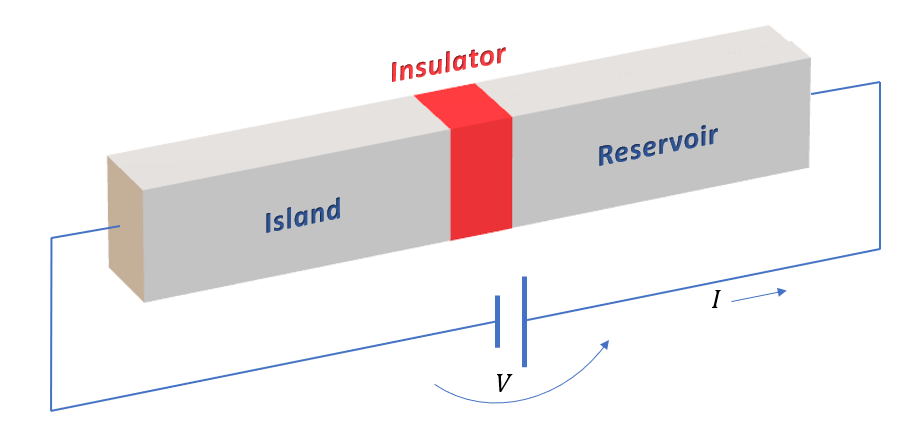
\includegraphics[width=0.7\textwidth]{pic/transmon/jj1.png}
\caption{Josephson Junction connected to a voltage source}
\label{fig:jj1}
\end{figure}

When the junction is cooled down below its critical temperature $Tc$ the behaviour of the component dramatically changes. By specific kind of interaction among couple of electrons with the lattice cooper pairs are formed. This effective particles, with bosonic character, can flow inside the superconductors without encountering any kind of resistance.\\
Let's suppose to write the two Ginzburg-Landau order parameter associated to the two superconducting regions:
\begin{equation}\begin{split}
\psi_{A} = \sqrt{n_{A}}\exp{i\phi_{A}}\\
\psi_{B} = \sqrt{n_{B}}\exp{i\phi_{B}}
\end{split}\end{equation}
which could be interpreted as the wave functions describing the behaviour of cooper-pairs. Considering a constant Voltage applied $V$ across the junction the energy difference for each cooper-pair will be $2eV$.
The Schroedinger equation for this system will be:
\begin{equation}
    \begin{split}
        i\hbar\frac{\partial \psi_{A}}{\partial t} = eV\psi_{A} + K\psi_{B}\\
        i\hbar\frac{\partial \psi_{B}}{\partial t} = eV\psi_{B} + K\psi_{A}
    \end{split}
\end{equation}

From this starting setting we could derive the final relations:
\begin{gather}
     I = \frac{dn_A}{dt} = \frac{2\sqrt{n_An_B}}{\hbar} Ksin(\delta)\\
    \frac{d\delta}{dt} = \frac{2eV}{\hbar} 
\end{gather}
 where $I$ is the current flowing inside the junction, $n_A, n_B$ the cooper-pair density associated to the superconducting junctions and $\delta$ is defined as the phase difference of the Ginzburg-Landau parameter along the junction:
 \begin{equation}
     \delta = \phi_{A} - \phi_{B} 
 \end{equation} 
 
 
 
\section{Cooper Pair Box}

\begin{figure}[h]
\centering
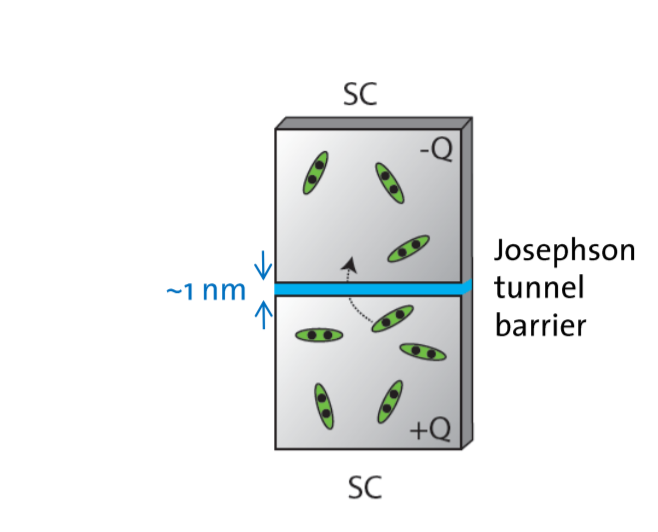
\includegraphics[width=0.4\textwidth]{pic/transmon/jj3.png}
\caption{Cooper pairs tunneling the Josephson junction}
\end{figure}
Starting from this macroscopic introduction, let's study how to write the main form of the Hamiltonian for a Josephson junction subject to a Voltage across it.
We could label the two superconducting areas of the Junction respectively 'Island' and 'Reservoir'. When we apply a constant Voltage electrons can be transferred from the reservoir to the island by tunneling through the thin layer of insulator.\\
We suppose that both the island and reservoir behaves as good BCS superconductors which requires the following condition to be respected $$\Delta << K_BT,\frac{e^2}{2C_{\Sigma}} $$ where $\Delta$ is the superconducting energy gap, $K_BT$ is the thermal fluctuations energy, $\frac{e^2}{2C_{\Sigma}}$ Coulomb energy of the island.\\ \par 
Under this condition we could suppose all electrons are paired and have become cooper-pairs.
We could now focus on the number of cooper-pairs contained inside the island in excess with respect to the reservoir \textbf{n} which is linked to the total charge though  $q = -2ne$ . \footnote{$n$ could assume integer values. If $n = 0$ then we would have charge neutrality across the junction.}\\ 
Since cooper pairs in the island could fluctuate by quantum tunneling between island and reservoir we will describe $n$ by its quantum operator $$n \rightarrow \hat{n}$$
with basis-eigenstates 
\begin{equation}
    \hat{n}\ket{n} = n\ket{n}
\end{equation}

Moreover to describe the condensate wave function of cooper-pairs  it will  be useful also to define the phase operator 
\begin{equation}
\delta \rightarrow \hat{\delta}
\end{equation} 

and an alternative state basis 

\begin{equation} 
\ket{\delta} =  \sum_{n= -\infty}^{\infty} e^{in\delta}\ket{n}
\end{equation}

Performing more detailed calculation (see Appendix) it is possible to obtain the following useful relations:
\begin{equation}
    \begin{split}\label{eq:delta}
        e^{i\hat{\delta}} = \sum_{n= -\infty}^{\infty} \ket{n}\bra{n+1}\\
        e^{-i\hat{\delta}} = \sum_{n= -\infty}^{\infty} \ket{n+1}\bra{n}\\
    \end{split}
\end{equation}
\begin{equation}
    \label{eq:delta1}
    \hat{n} = \frac{1}{i}\frac{\partial}{\partial\delta}
\end{equation}

\subsection{Tunneling Hamiltonian}
In order to model the tunneling behavior of cooper-pairs across the junction we could define the following effective Hamiltonian

\begin{equation}
    H_J = -\frac{E_J}{2}\sum_{n=-\infty}^{\infty} (\ket{n}\bra{n+1} +\ket{n+1}\bra{n})
\end{equation}

Using eq. \ref{eq:delta} it is possible to rewrite the Hamiltonian as

\begin{equation}
    H_J = -\frac{E_J}{2}(e^{i\hat{\delta}}+e^{-i\hat{\delta}}) = -\frac{E_J}{2}cos(\hat{\delta})
\end{equation}


\subsection{Electrostatic Hamiltonian}
Let's now have a look to the circuital sketch of the Josephson junction in fig. \ref{fig:jj2}. Considering the electrostatic energy of cooper-pairs we could write an Hamiltonian of the form:
\begin{figure}[h]
\centering
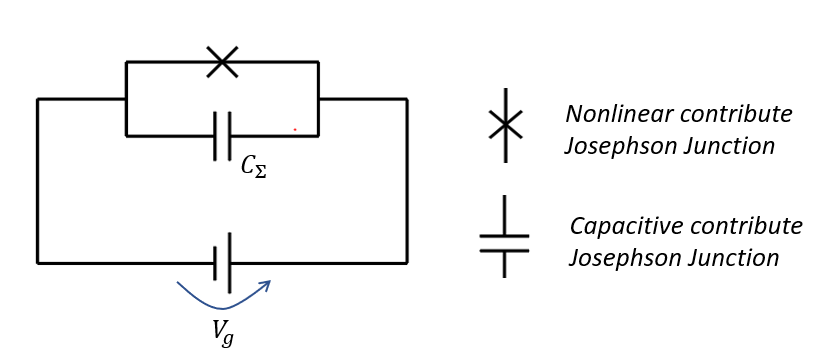
\includegraphics[width=0.7\textwidth]{pic/transmon/jj2.png}
\caption{Josephson Junction circuital sketch}
\label{fig:jj2}
\end{figure}



$$H_{el} = \frac{(2e)^2}{2C_{\Sigma}}\hat{n}^2 + 2e\hat{n}V_g  = 4E_C(\hat{n}-n_g)^2$$
   
with $E_C = \frac{e^2}{2C_{\Sigma}}$ and $n_g = \frac{C_{\Sigma}V_g}{2e}$ the number of cooper-pairs induced charge by the constant voltage $V_g$, and $C_{\Sigma}$ the total capacitance associated to the junction.\\
Actually what could happen, in general, is that we are never able to control exactly the value of $V_g$, due either to the presence of uncontrollable charge fluctuactions or noise. We describe in general $n_g$ as
\begin{equation}
    n_g = \frac{Q_r^2}{2e} + \frac{C_{\Sigma}V_g}{2e}
\end{equation}
where $Q_r$ represents the environment-induced offset charge.


\section{Solving the complete Hamiltonian}
Now let's compose all the parts to obtain the final Hamiltonian of the Cooper-pair box in phase representation
\begin{equation}
    \label{HamiltonianJJ}
    \begin{split}
    H = 4E_C(\hat{n}-n_g)^2 -E_Jcos(\hat{\delta}) \\= 4E_C(\frac{1}{i}\frac{\partial}{\partial\delta}-n_g)^2 -E_Jcos(\hat{\delta})
    \end{split}
\end{equation}
where we obtained the last equality using eq. \ref{eq:delta1} .\\
This would lead to the following Schrodinger equation
\begin{equation}
    4E_C(\frac{1}{i}\frac{\partial}{\partial\delta}-n_g)^2 -E_Jcos(\hat{\delta})\Psi(\delta) = E\Psi(\delta)
\end{equation}

As showed in more details in Appendix it is possible to solve this equation Mathieu functions obtaining the following result
\begin{equation}
    \Psi(\delta) = e^{in_g\delta}g(\frac{\delta}{2})\\
\end{equation}
where $g(\delta)$ could be obtained by solving the following differential equation
\begin{equation}
    g^{\prime\prime}(x) + [\frac{E}{E_C} + \frac{E_J}{E_C}cos(2x)]g(x) = 0
\end{equation}

We could also calculate the eigenergies (details in Appendix) which will  be given by
\begin{equation}
    E_m(n_g) = E_Ca_{[2n_g+k(m,n_g)]}(-\frac{E_J}{2E_C})
\end{equation}
with $a_x(y)$ Mathieu's characteristic value and $k(m,n_g)$ a function properly sorting the eigenvalues.\\
Plots the first eigenenergies $E_0(n_g), E_1(n_g),E_2(n_g)$ for different values of the ratio $E_J/E_C$ are shown in fig. \ref{fig:transmon}. 
\begin{figure}[h]
\centering
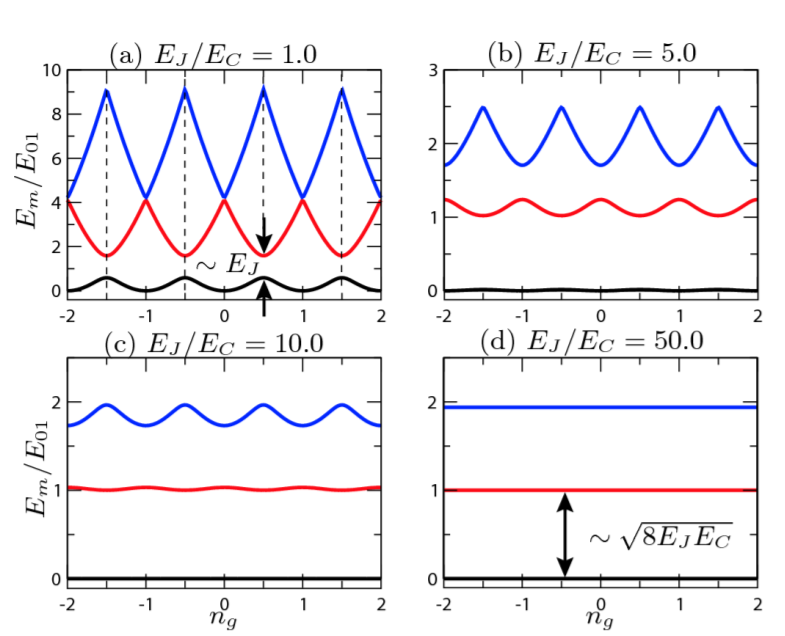
\includegraphics[width=0.7\textwidth]{pic/transmon/jj4.png}
\caption{Eigenenergies $E_0, E_1,E_2$ as a function of the offset charge  $n_g$ with different ratios of $E_J/E_C$. Energies are normalized with respect to $E_{01}$. Picture from \href{https://doi.org/10.1103/PhysRevA.76.042319}{Koch et al. PRA 2007}}
\label{fig:transmon}
\end{figure}

It is worth noticing that
\begin{itemize}
    \item the anharmonicity of the junction depends on the ratio $E_J/E_C$
    \item the eigenenergies fluctuations wrt to $n_g$ decrease very rapidly as $E_J/E_C$ increases
\end{itemize}
Having a high anharmonicity would help us in addressing selectively the $\ket{0} \longleftrightarrow \ket{1}$ while having small eigenergies fluctuations would stabilize the energy levels with respect to some external noise changing $n_g$


\section{Transmon regime}
The sensitivity of the qubit with respect to the charge offset fluctuations $n_g$ is important for increasing the coherence time $T_2$ of the qubit as mushc as possible. In view of this working in the transmon regime is of vital importance. The transmon regime is defined when the condition $$\frac{E_J}{E_C} >> 1$$  is met.\\ Let's now focus on the main consequences of working in this regime.
By performing some more detailed calculations, which go beyond the aim of this report, we could approximate energy eigenvalues, in the large limit of $E_J/E_C$, as \begin{equation}
    E_m \simeq E_m(n_g = 1/4) - \frac{\epsilon_m}{2}cos(2\pi n_g)
\end{equation}
with 
\begin{equation}
    \epsilon_m =  E_m(n_g = 1/2)- E_m(n_g = 0)
\end{equation}
and
\begin{equation}
    \epsilon_m \propto e^{-\sqrt{8E_J/E_C}} 
\end{equation}
This result is important as it effectively shows that if we are in the transmon regime energy fluctuations would get exponentially suppressed suppressed. \\
Let's try now to derive the anharmonic Hamiltonian associated to the transmon regime. In fig. \ref{fig:transmon2} you could see the plot of the cosine potential $-E_Jcos(\delta)$ of the Josephson junction Hamiltonian presented in eq. \ref{HamiltonianJJ}. When we consider the transmon lowest energy levels $E_0, E_1$ we can affirm that we would be in the condition $$\left\langle\delta^2 \right\rangle \ll 1$$ which tells us that $\delta$ tends to assume very small values for fundamentals levels
\begin{figure}[h]
\centering
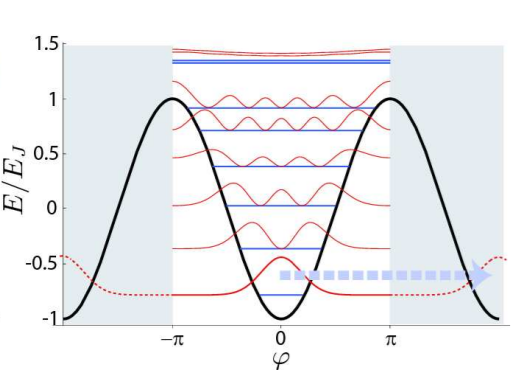
\includegraphics[width=0.5\textwidth]{pic/transmon/jj5.png}
\caption{Cosine potential with eigenenergies and squared moduli of the eigenfunction.Picture from \href{https://doi.org/10.1103/PhysRevA.76.042319}{Koch et al. PRA 2007}}
\label{fig:transmon2}
\end{figure}

This important condition allows us to approximate cosine potential as 
\begin{equation}
    -E_Jcos(\hat{\delta}) \simeq -E_J + E_J\frac{\hat{\delta}^2}{2} -E_J\frac{\hat{\delta}^4 }{4!} + ...
\end{equation}
So, supposing $n_g \simeq 0$, we could approximate the Hamiltonian of qe \ref{HamiltonianJJ} as
\begin{equation}
    H \simeq 4E_c\hat{n}^2 + E_J\frac{\hat{\delta}^2}{2} -E_J\frac{\hat{\delta}^4 }{4!}
\end{equation}
and by redefining the operators $\hat{n}$ and $\hat{\delta}$ as
\begin{equation}
    \begin{split}
        \hat{n} = n_0(\hat{a} + \hat{a}^+)\\
        \hat{\delta} = i\delta_{0}(\hat{a}^+ - \hat{a})
    \end{split}
\end{equation}
we could obtain the final form of the Hamiltonian (see Appendix)
\begin{equation}
\label{HamiltonianSimplified}
    \begin{split}
        H = \hbar\omega\hat{a}^+\hat{a} + \frac{\hbar\alpha}{2}(\hat{a}^+)^2(\hat{a})^2\\ \\
        \omega = \sqrt{8E_CE_J} - E_C \\  \alpha = \frac{E_C}{\hbar} 
        \end{split}
\end{equation} 

\section{Squids: a couple of words}
Up to this moment we have only analysed what happens to a single Josephsonn junction circuit. However, as it could be seen from eq. \ref{HamiltonianSimplified} the value of $\omega$ is depending on $E_C$ and $E_J$ which are fixed once we produce the junction. This situation presents two back-draws:
\begin{itemize}
    \item $\omega$ could not be precisely determined since production processes does not allow us to have enough precision nor over $E_C$ nor $E_J$ 
    \item $\omega$ can not be dynamically changed and this would be problematic for performing two qubit gates
\end{itemize}
In order to overcome these limitations Squids (Superconducting Quantum Interference Devices) were introduced. Fig. illustrates what is the circuital structure of Squids: they are composed by two, usually identical, Josephson junction in parallel. This introduces a superconducting loop into the circuit whose properties could be controlled with the aid of an external magnetic field $\Vec{B}$.
If we consider the flux associated to the closed path composed by the two junctions we could write:
\begin{equation}
    \hat{\phi_1}-\hat{\phi_2} +\frac{\Phi_{ext}}{\phi_0} = 2\pi m
\end{equation}
with $\phi_{1,2}$ the phase associated to each junction respectively, $\Phi_{ext}$ the flux of the external magnetic field through the two junction closed path, $\phi_0$ the quantum flux and $m \in \mathbb{Z}$.
Through some more detailed calculations it would be possible to show that it is possible to obtain a system that behaves like a single junction and that has a different tunneling Hamiltonian  
\begin{equation}
\begin{split}
    H_J = -2E_J|cos(f/2)|cos(\hat{\phi})\\ \\
    f = \Phi_{ext}/\phi_0\\
    \hat{\phi} = \frac{\hat{\phi_1} +\hat{\phi_2}}{2}
    \end{split}
\end{equation}


It is important to notice that now the tunneling energy $E_J\prime$ could be tuned at will by just changing the external flux that goes through the junction loop:
\begin{equation}
    E_J\prime = E_J|cos(f/2)|
\end{equation}
So Squids are able to guarantee more flexibility and tunability in situ also while the experiment is in progress

\begin{figure}[h]
\centering
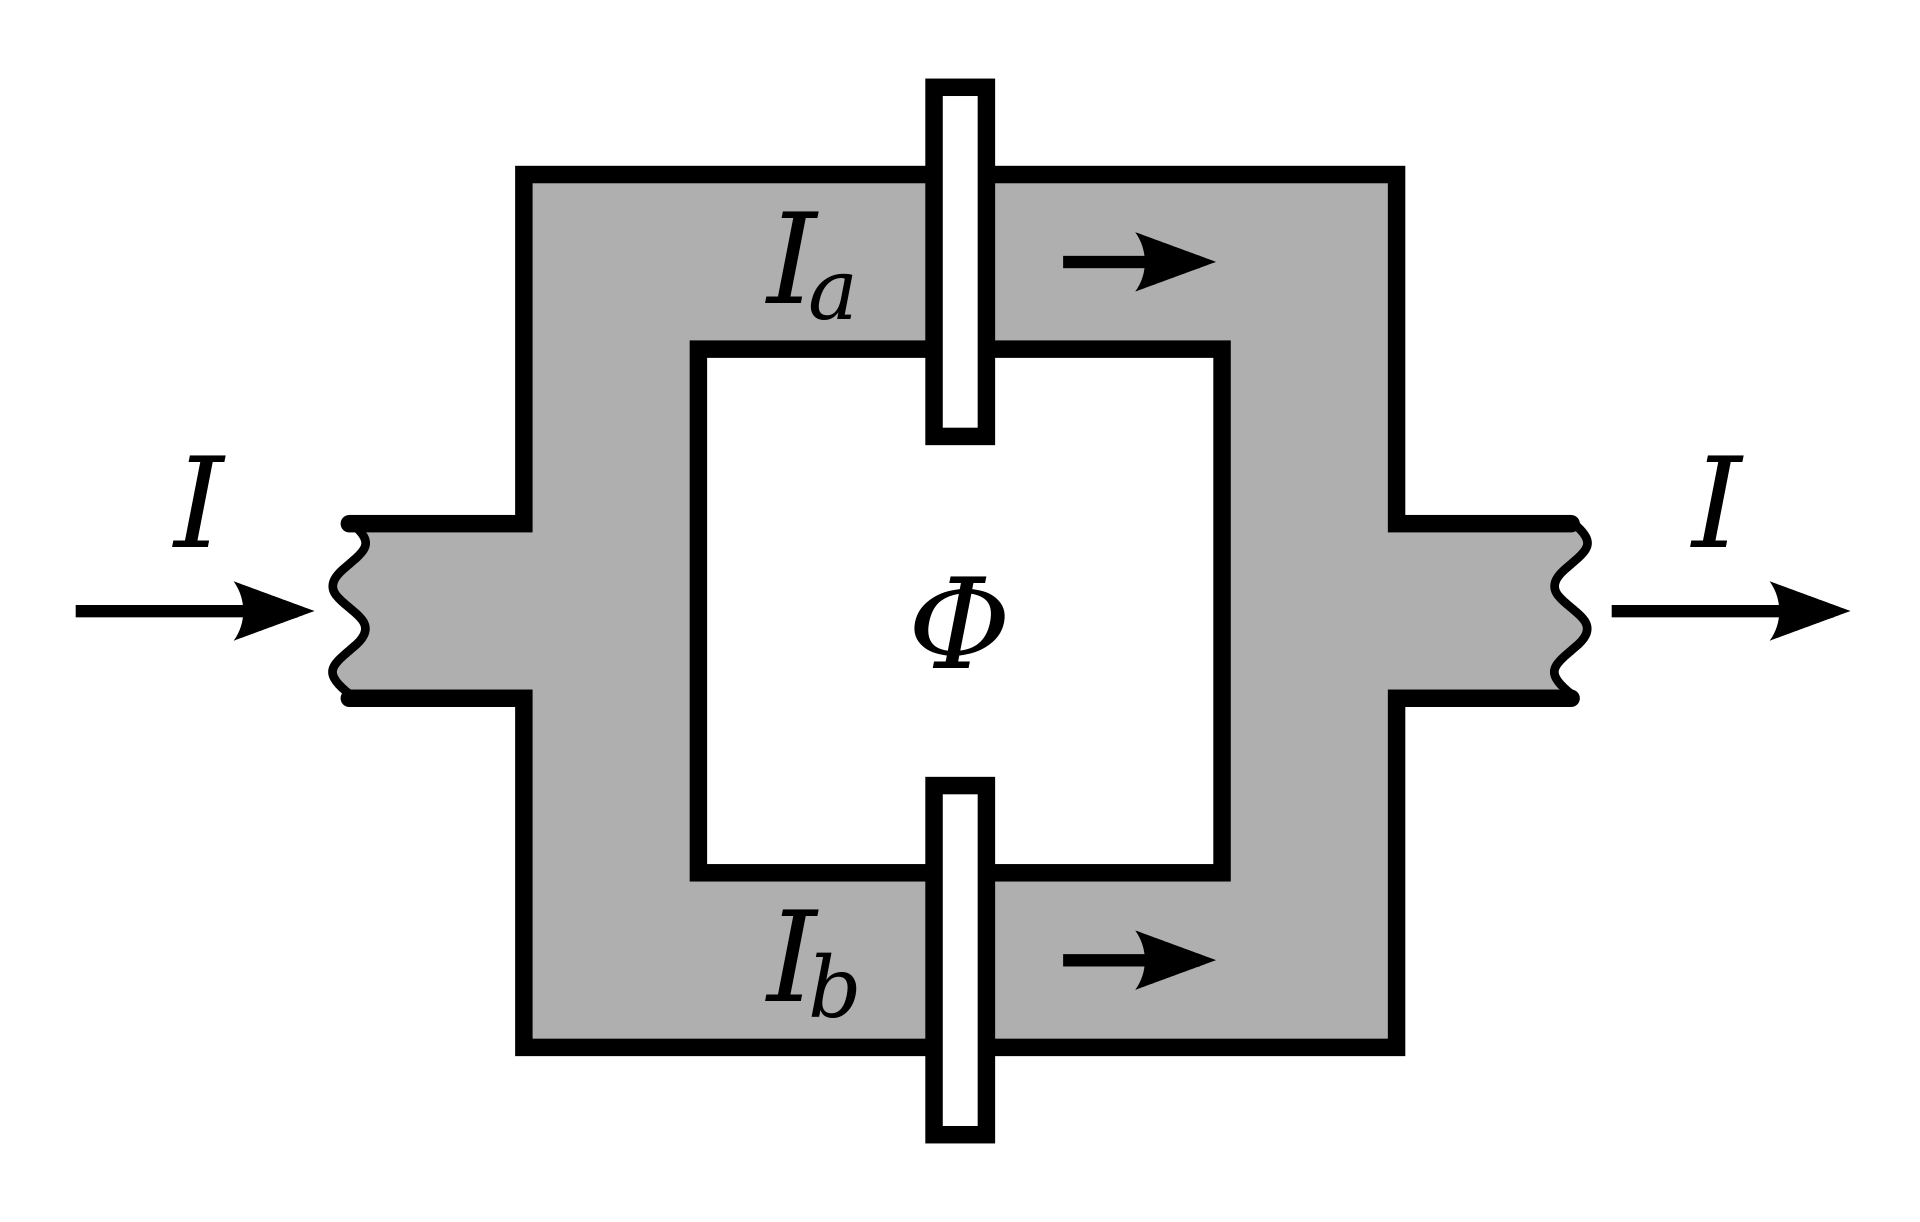
\includegraphics[width=0.3\textwidth]{pic/transmon/squid1.png}
%\caption{SQUID structure from \hyperlink{https://it.wikipedia.org/wiki/SQUID}{Wikipedia} }
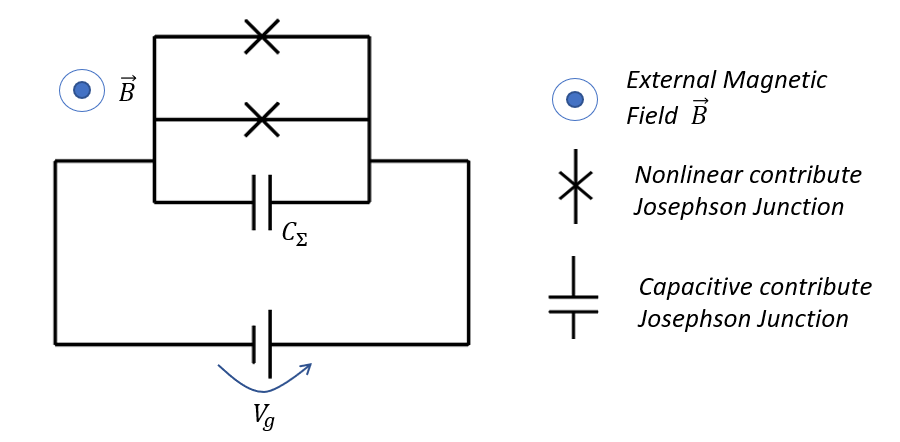
\includegraphics[width=0.7\textwidth]{pic/transmon/squid2.png}
\caption{SQUID circuital sketch}
\label{fig:squid1}
\end{figure}

\section{Transmon qubit in a 3d cavity}
After introducing, transmon qubit Hamiltonian let's have a look at the practical realization that was chosen for this project. In order to simplify as mushc as possible the practical implementation of the device it was chosen to produce a transomn qubit in a 3d cavity. The main structure is shown in fig. \ref{}. We can see:
\begin{itemize}
    \item the transmon chip deposited over a sapphire substrate
    \item the electromagnetic cavity 
\end{itemize}
The cavity is implemented for trapping electromagnetic fields inside the cavity. We can study the interaction of the qubit with the stationary electromagnetic modes in a really controlled fashion and achieve particular working conditions as the dispersive regime. Let's focus now on the transmon chip.
\subsection{Transmon}
A more detailed structure of the transmon chip could be seen in fig. 
It shows a Squid structure (two Josephson Junction in parallel) connected to a two extremal conductive pads called respectively 'Island' and 'Reservoir' also made by the same superconductive material used for the josepshon junction. The presence of the pads is necessary as:
\begin{itemize}
    \item it increases the dipole associated to the transmon which contributes to a stronger coupling with the electormagnetic modes
    \item it increase the total capacitance of the qubit $C_{\Sigma}$ and so it contributes entering \footnote{Remember than $E_C = \frac{e^2}{2C_{\Sigma}}$ so as long $C_{\Sigma}$ increases $E_C$ decreases and we enter a 'deeper' transmon regime ($E_J/E_C \gg 1$) the strong coupling regime}
\end{itemize}
Let's first focus on the capacitance calculations and circuital structure which is shown in picture \ref{}. Notice that since the transmon is inserted inside a 3d electromagnetic cavity we have to consider also the capacitive interaction between the two. The complete effective capacitance will then be:
\begin{equation}
C_{\Sigma} = 2C_J + C_{I-R} + \left(\frac{1}{C_{R-C}} + \frac{1}{C_{I-C}}\right)^{-1}
\end{equation}
where $C_J$ is the Josephson junction capacitance, $C_{I-R}$ the capacitance between the Island and Reservoir, $C_{R-C}$ the capacitance between the Reservoir pad and the cavity, $C_{I-C}$ the capacitance between the island and cavity.\\
\par
Now let's have a look to dipole calculation. Since the dimensions ($~\mu m$)of the transmon are very small if compared with the cavity ones ($~mm$) we could consider the Electric field to be constant across all the qubit. Let's suppose $E(y) = E_0$ is parallel to the pads as represented in fig. Now we could also associate a potential to it, namely, $V(\vec(r)) = -E_0\cdot y$. The electric field induces a charge with the same modulus but opposite sign, over the transmon islands and reservoir$Q = - Q_{r} = Q_I$ We could then write the interaction Hamiltonian as:
\begin{equation}
    H_{int} = \int_{V} \rho(\vec{r})\,V(\vec{r})\,d\vec{r} = -E_0\, Q\, d_{t}
\end{equation}
where $V$ is the volume of the transmon, $\rho(\vec{r})$ is the charge density defined over all the transmon volume, Q is the total charge $d_{t}$ is the effective distance associated to the transmon and $Qd_{t}$ the effective dipole.
It should be noted that in this analysis we did not consider the presence of the two Josephson junctions. This is mainly due to the difficulty arisen in simulating the charge distribution over the Josephson junction. It would be possible to estimate roughly the effect of the junction with the following formula:
\begin{equation}
    d_t\prime = \frac{Q_J\,d_J+Q\,d_t}{Q_J + Q}
\end{equation}
with $Q_J$  and $d_J$the charge and effective distance associated to the junction. We performed some calculation starting from cad simulation result and it was possible to see that the effect of the junctions is really negligible.
We could finally write the quantum transmon Hamiltonian as:
\begin{equation}
    H_{int} =-\hat{E_0} \, \hat{Q} \, d_t = E_0\,(\hat{a} + \hat{a}^+)\, Q\, d_t\,\frac{\hat{b}^+- \hat{b}}{\sqrt{2}} = \hbar \sum_{i,j} g_{ij} \ket{i}\bra{j}(\hat{a} + \hat{a}^+)
\end{equation}
where $$\hat{Q} = Q\,\frac{\hat{b}^+- \hat{b}}{\sqrt{2}} = i\left(\frac{E_J}{8E_C}\right)^{1/4}\frac{\hat{b}^+- \hat{b}}{\sqrt{2}}$$ is the quantum charge operator, $$\hat{E}=E_0\,(\hat{a} + \hat{a}^+)$$ the electric field operator and $\ket{i}$ indicates a generic transmon level.
It is interesting to notice that
\begin{equation}
    \begin{split}
        \hbar\,g_{ij} = E_0\,Q\,d_t\,\bra{i}\left(\frac{\hat{b}^+- \hat{b}}{\sqrt{2}}\right)\ket{j}
    \end{split}
\end{equation}
By performing more detailed calculation \footnote{For acquiring a deeper insight over this section consult \hyperlink{https://arxiv.org/pdf/cond-mat/0703002.pdf}{Koch et al.}} in the large transmon limit ($ E_J/E_C \gg 1$) it is possible to obtain
\begin{equation}
    \begin{split}
        |\bra{j+1}\hat{n}\ket{j}| \approx \sqrt{\frac{j+1}{2}}\left(\frac{E_J}{8E_C}\right)^{1/4}\\
        |\bra{j+k}\hat{n}\ket{j}| \rightarrow 0  
    \end{split}
\end{equation}
So supposing that we have can have dipole transition only among subsequent levels and considering only the two fundamental levels of the transmon as $\ket{g} \: \ket{e}$ we could write
\begin{equation}
    H_{qubit} = \hbar\, \omega_{eg}\, \hat{a}^+\hat{a} + \hbar\, g_{eg}\, \hat{\sigma_x}\, (\hat{a} + \hat{a}^+)
\end{equation}
The practical calculations of both dipole and capacity are discussed in next chapters.
